\subsection{Model Architectures}

To provide a comprehensive understanding of the neural network architectures used in our experiments, we present visual diagrams of each model design. These diagrams illustrate the layer configurations, connections, and key architectural features that distinguish each model.

\subsubsection{Small CNN Architecture}

Our custom Small CNN architecture represents a lightweight convolutional neural network designed specifically for this research. Figure~\ref{fig:small_cnn_arch} illustrates its structure with both single-neuron and dual-neuron output configurations.

\begin{figure}[htbp]
\centering
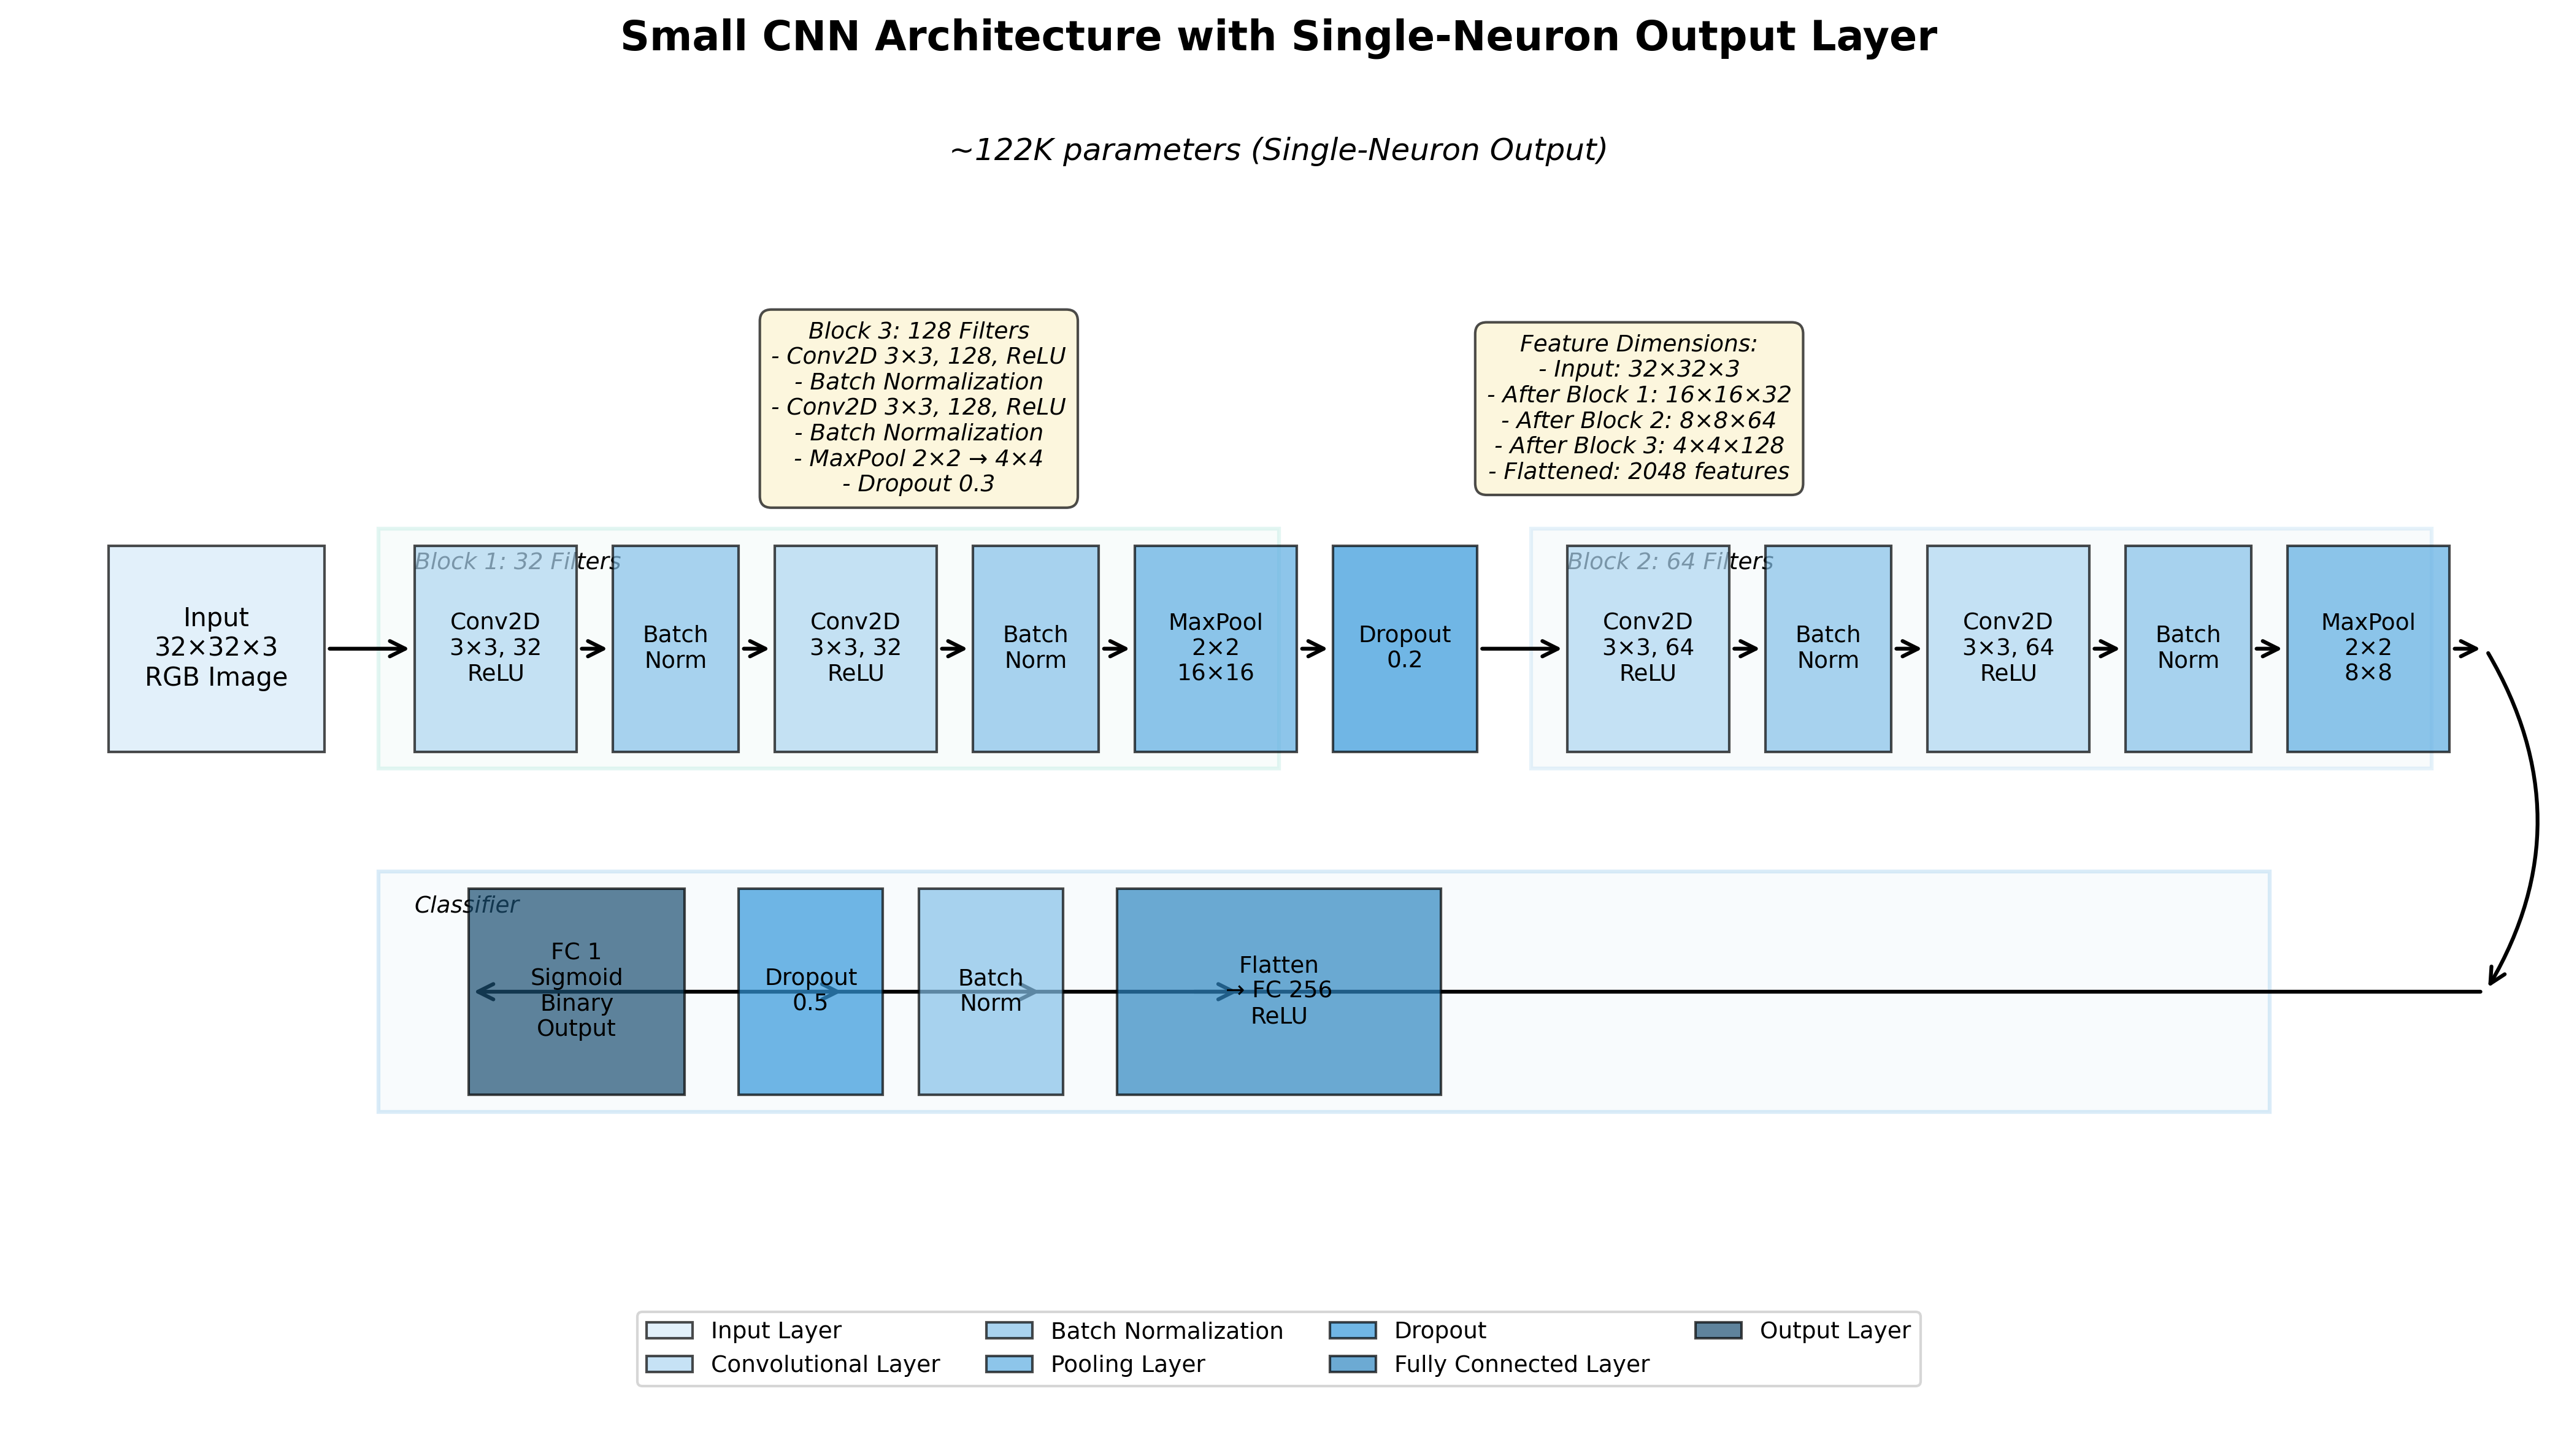
\includegraphics[width=\textwidth]{figures/small_cnn_1neuron_architecture.png}
\caption{Small CNN architecture with single-neuron output layer. The network consists of three convolutional blocks followed by fully connected layers and a single sigmoid output neuron.}
\label{fig:small_cnn_arch}
\end{figure}

The Small CNN architecture features:
\begin{enumerate}
\item Three convolutional blocks, each containing two convolutional layers with batch normalization, followed by max pooling and dropout
\item A fully connected layer with 256 neurons, batch normalization, and dropout
\item Either a single-neuron output with sigmoid activation or a dual-neuron output with softmax activation
\end{enumerate}

This architecture provides a baseline model with approximately 813,000 parameters, all of which are trainable during our experiments.

\subsubsection{ResNet50 Architecture}

For our second architecture, we employed the ResNet50 model with transfer learning. Figure~\ref{fig:resnet50_arch} shows the architecture with its characteristic residual connections.

\begin{figure}[htbp]
\centering
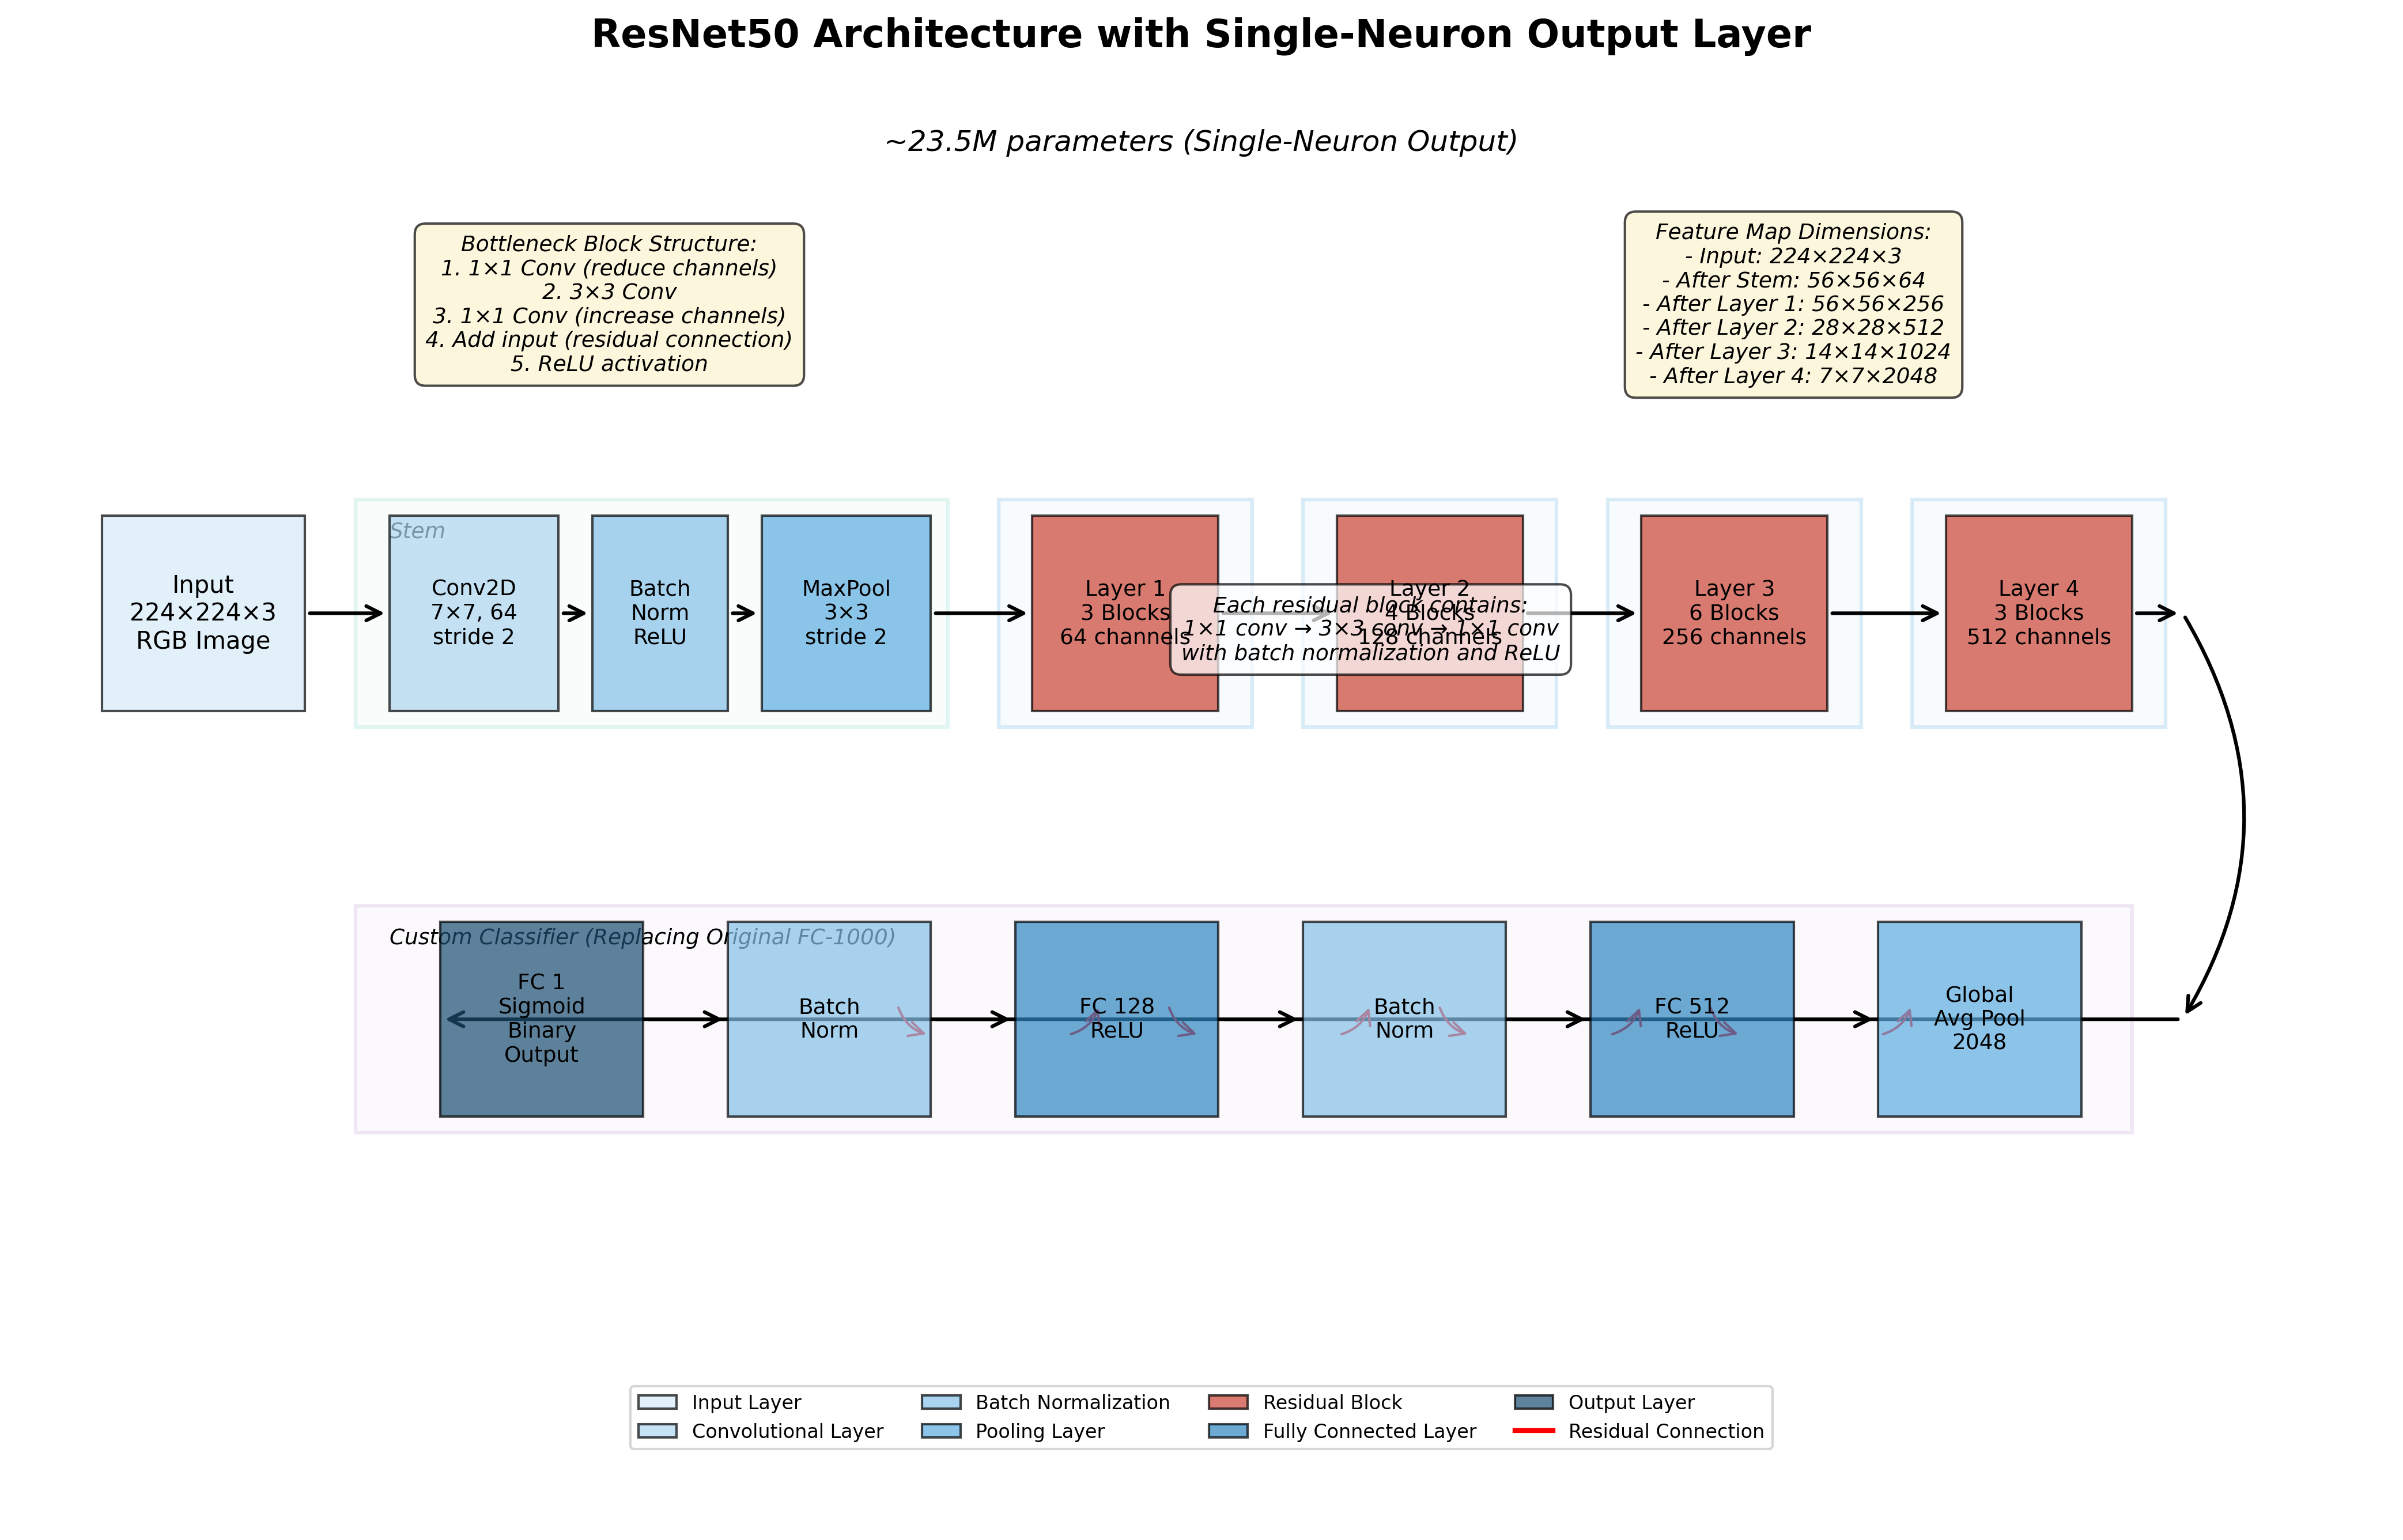
\includegraphics[width=\textwidth]{figures/resnet50_1neuron_architecture.png}
\caption{ResNet50 architecture with single-neuron output layer. The model utilizes pre-trained weights from ImageNet, with only the final residual block and classifier layers fine-tuned for our binary classification tasks.}
\label{fig:resnet50_arch}
\end{figure}

Key features of our ResNet50 implementation include:
\begin{enumerate}
\item Pre-trained weights from ImageNet classification
\item Frozen early layers (all except layer4 and the classifier)
\item Custom classifier with two fully connected layers (512 and 128 neurons)
\item Either a single-neuron output with sigmoid activation or a dual-neuron output with softmax activation
\end{enumerate}

The ResNet50 model contains approximately 24.6 million total parameters, with 16.1 million of those being trainable in our transfer learning setup.

\subsubsection{Vision Transformer (ViT) Architecture}

Our third architecture is the Vision Transformer (ViT), which represents the attention-based paradigm in computer vision. Figure~\ref{fig:vit_arch} illustrates the ViT architecture with its distinctive transformer encoder blocks.

\begin{figure}[htbp]
\centering
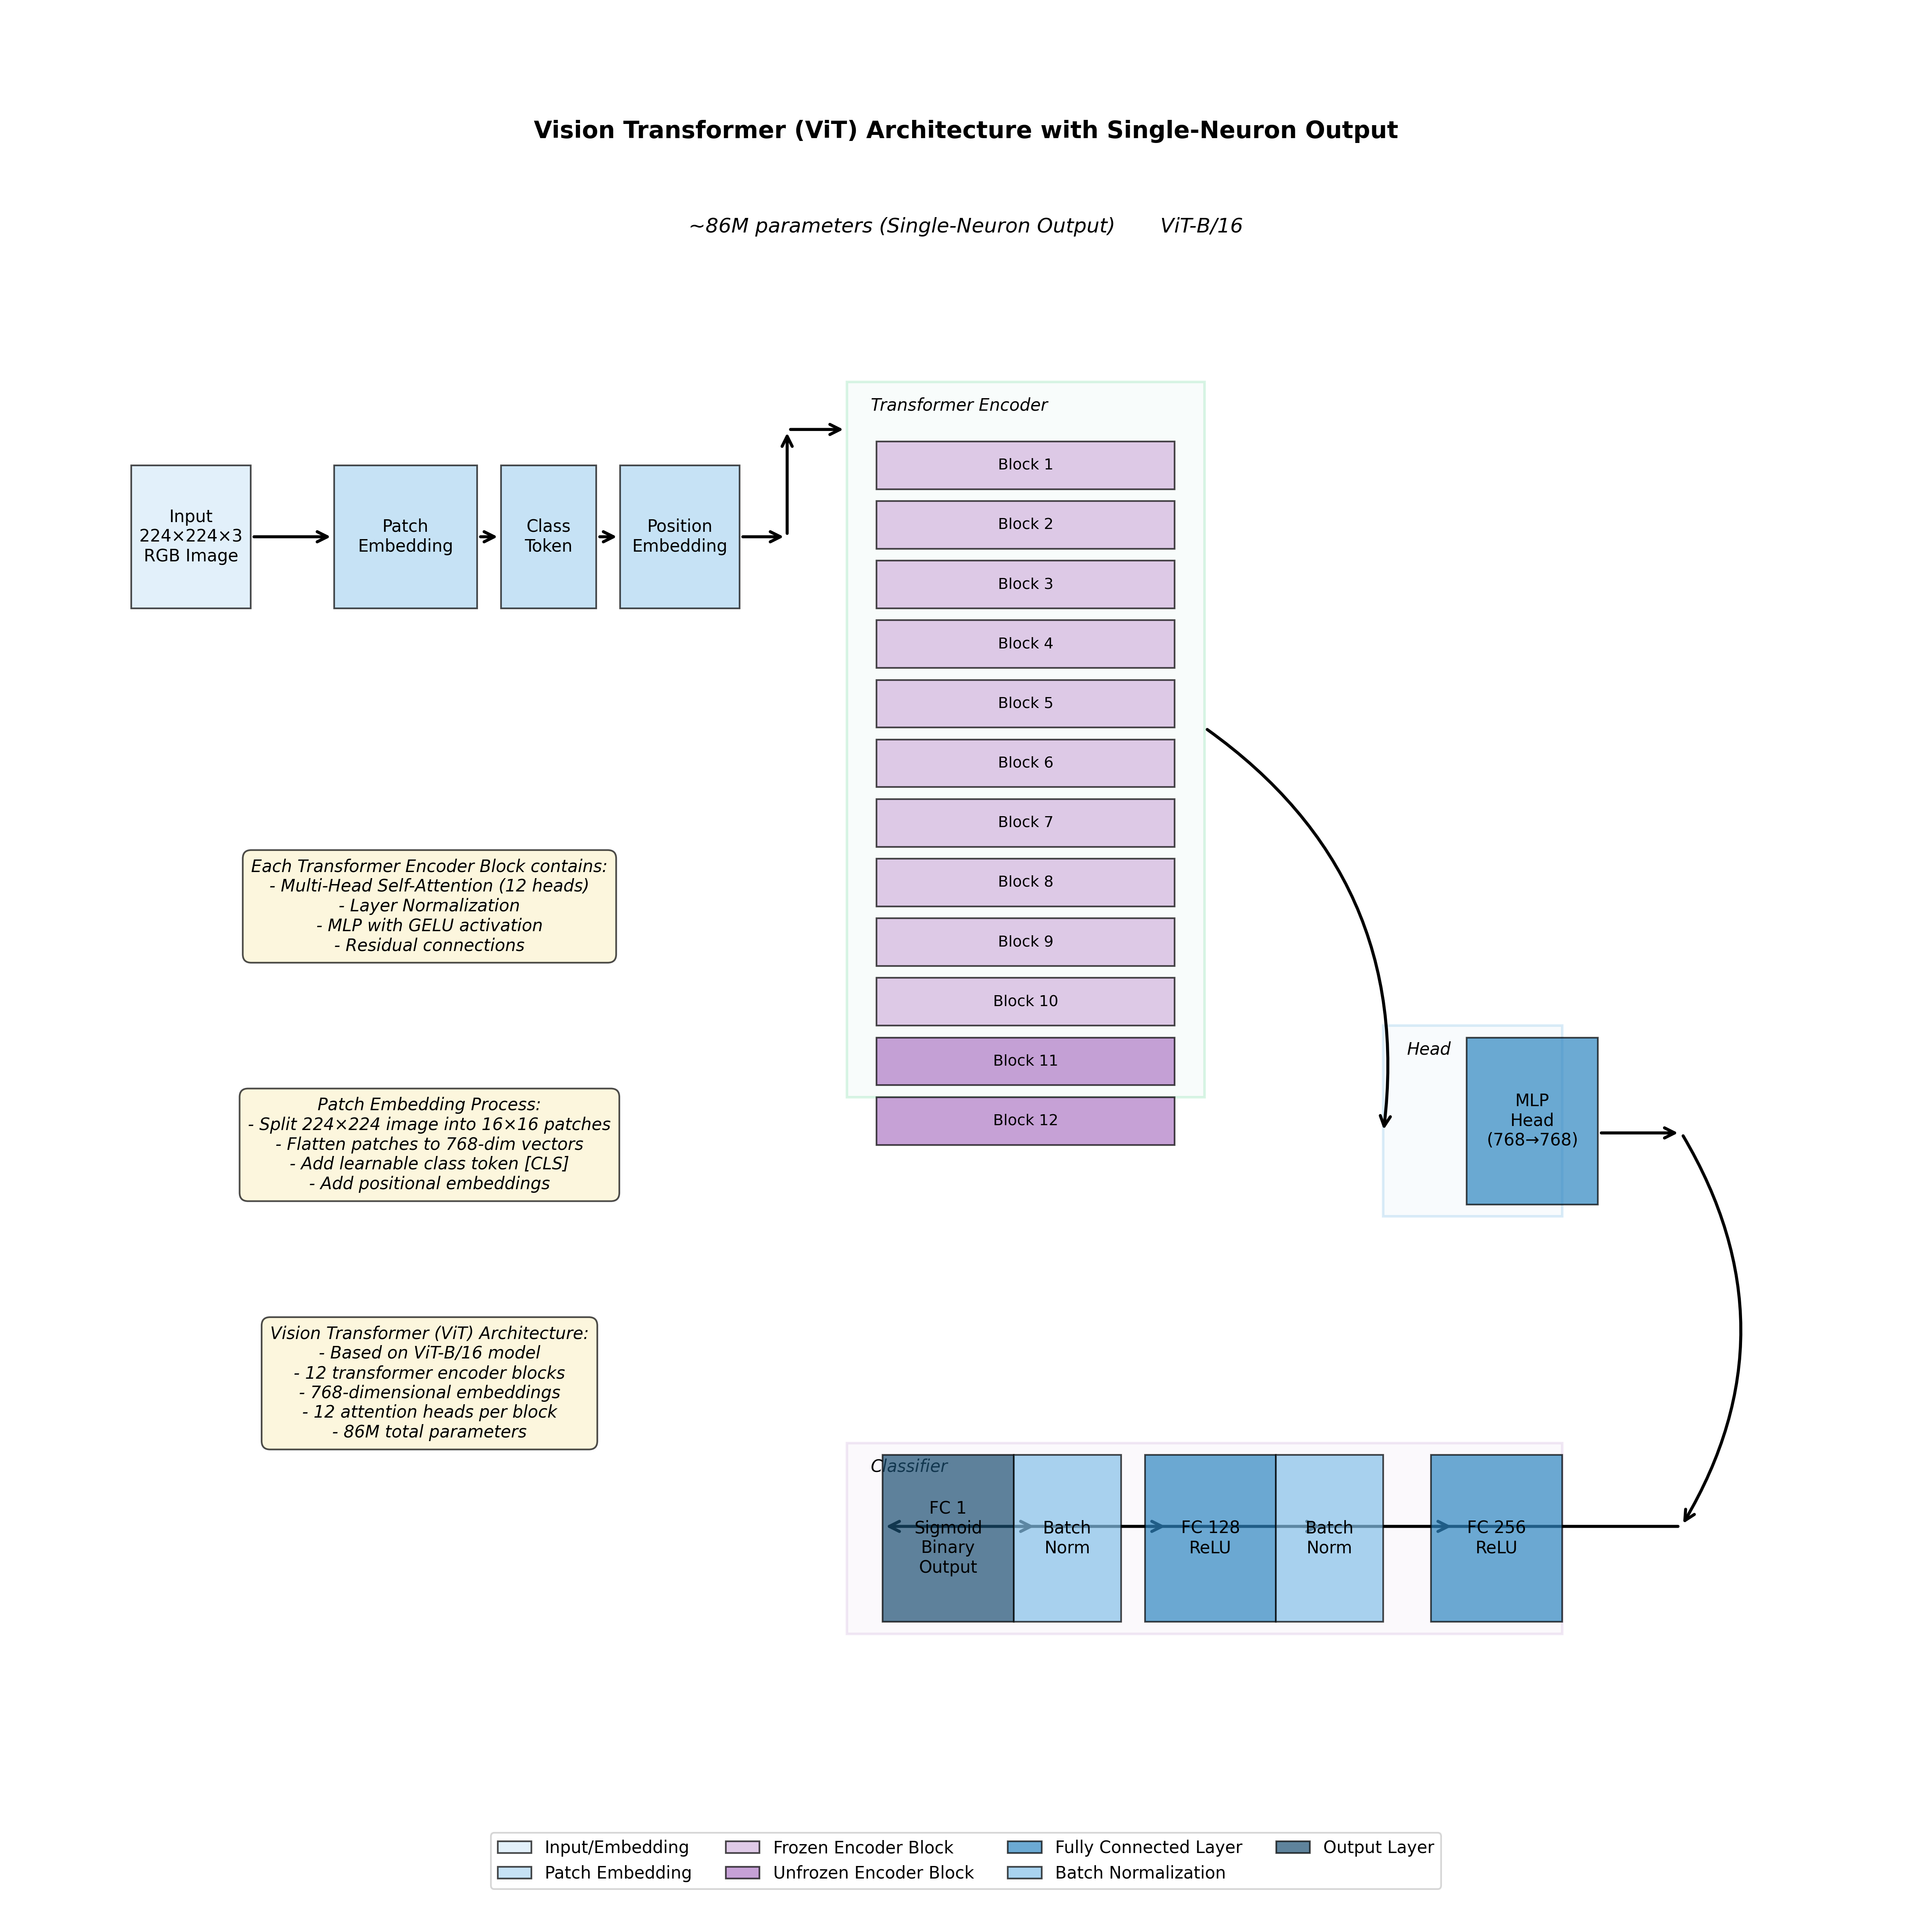
\includegraphics[width=\textwidth]{figures/vit_1neuron_architecture.png}
\caption{Vision Transformer (ViT) architecture with single-neuron output layer. The model divides the input image into patches, processes them through transformer encoder blocks, and uses the class token representation for classification.}
\label{fig:vit_arch}
\end{figure}

The ViT architecture features:
\begin{enumerate}
\item Patch embedding that divides the input image into 16×16 patches
\item A learnable class token that aggregates information for classification
\item 12 transformer encoder blocks with multi-head self-attention and MLP layers
\item Transfer learning with only the final two encoder blocks and classifier being fine-tuned
\item Custom classifier with two fully connected layers (256 and 128 neurons)
\item Either a single-neuron output with sigmoid activation or a dual-neuron output with softmax activation
\end{enumerate}

The ViT model is the largest in our study with approximately 86 million total parameters, though only about 230,000 of these are trainable due to our transfer learning approach.

\subsubsection{Output Layer Configurations}

For each architecture, we implemented two output layer configurations:

\begin{enumerate}
\item \textbf{Single-Neuron Configuration}: A single output neuron with sigmoid activation, where outputs closer to 0 represent one class and outputs closer to 1 represent the other class. The loss function used is Binary Cross Entropy.

\item \textbf{Dual-Neuron Configuration}: Two output neurons with softmax activation, where each neuron represents the probability of the input belonging to one of the two classes. The loss function used is Cross Entropy.
\end{enumerate}

As shown in our parameter analysis, the difference in parameter count between these two configurations is minimal (less than 0.1\% increase), ensuring that performance differences can be attributed to the architectural choice rather than model capacity.
